\newpage
\subsection{The storage system}

\begin{figure}[!h]
    \centering
    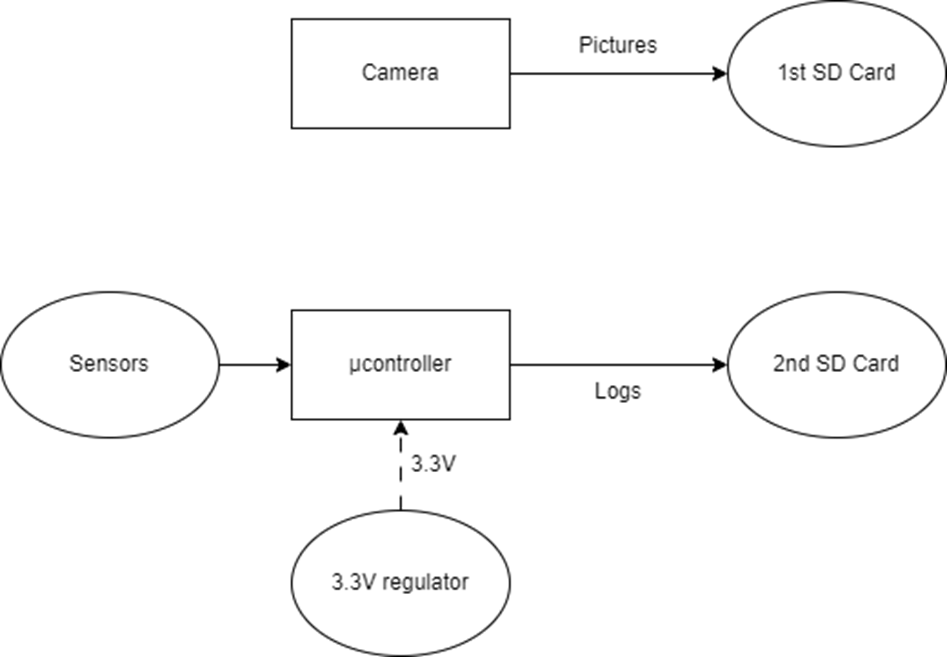
\includegraphics[width=0.9\textwidth]{\currfiledir/figures/storage_diagram.png}
    \caption{Storage system diagram}
\end{figure}
The storage system is made of a SD card linked to the camera and a second SD card linked to the microcontroller. The first SD card linked to the camera is used to store the pictures taken by the camera. The second one is used to store the logs emitted by the system.
The measures gathered by the sensors are fetched by the microcontroller, which sends them via LoRa to the gateway and stores them at the same time in the 2nd SD card.